\subsection{Problem 5(1.13)}
\textbf{What's the maximum number of regions definable by n zig-zag lines, each of which consists of two parallel infinite half-lines joined by a straight segment?}
\begin{figure}[h]
  \centering
  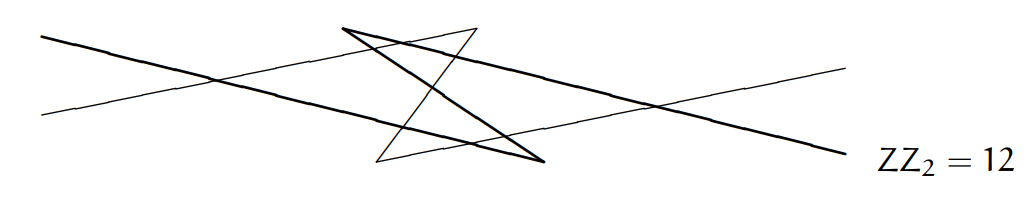
\includegraphics[width=0.7\textwidth]{images/1-13-zig-zag.PNG}
  \label{fig:example}
\end{figure}
\par

\begin{flushleft}
\textbf{Solution: }
\par
After a little thought, we realize that a zig zag is like three intersecting lines. Three intersecting line creates 7 regions. But one zig zag only creates 2 regions. So we lose 5 a region per zig zag.
We know number of regions generated by $n$ lines is, $L_n=\frac{n(n+1)}{2}+1$

So, number of regions definable by $n$ zig-zay hes is,
$$
\begin{aligned}
Z Z_n & =L_{3 n}-5 n \\
& =\frac{3 n(3 n+1)}{2}+1-5 n \\
& =\frac{9 n^2+3 n}{2}+1-5 n \\
& =\frac{9}{2} n^2+\frac{3}{2} n-5 n+1 \\
& =\frac{9}{2} n^2-\frac{7}{2} n+1
\end{aligned}
$$
\end{flushleft}